\chapter{Background}\label{ch:Background}

\section{Graphs Embedding}
Graph data is usually highly dimensional and defined in a non-euclidean form. Hence, typical processing methods defined on euclidean spaces cannot be used on graph data. Graph embedding methods convert the graph data into a vector representation while trying to preserve original graph properties\cite{Cai2018}.%\cite{Chen2020, Cai2018}.
Graph embedding methods can be classified as node embedding, edge embedding, hybrid embedding, and whole graph embedding. In literature, a distinction is made between graph representation learning and graph embedding\cite{Cai2018, Chami2022}, where graph representation does not require the final vector to be low-dimensional. In this paper, we focus on whole graph embedding, where each entire graph is represented as a vector\cite{Maddalena2021}. The vector representation can be used to compare graph similarity for important tasks, including classification and clustering. The main challenges in whole graph embedding are how to capture the properties of a whole graph and how to make a trade-off between expressiveness and efficiency\cite{Cai2018}. Several methods have been proposed for whole graph embedding, including matrix factorization, deep learning, edge reconstruction, graph kernel, and generative models\cite{Cai2018, Maddalena2021}.

Graph2Vec is a popular neural network-based architecture for graph embedding\cite{Narayanan2017}. Some advantages of Graph2Vec are that the model is trained in an unsupervised manner, the learned model is task agnostic, the algorithm is data-driven, and resulting vectors capture structural equivalences. Graph2Vec utilizes the non-linear Weisfeiler-Lehman (WL) kernel, %\cite{weisfeiler1968reduction},
which is shown to outperform other linear kernels\cite{shervashidze2011weisfeiler}. %\cite{shervashidze2011weisfeiler, Yanardag2015}.
WL kernel is used to rename the nodes using a hash value that represents a rooted sub-graph on the given node. These sets of node names are viewed as a set of words in a document. The techniques from the Natural language processing (NLP) domain are borrowed for learning an embedding. Doc2Vec is based on Word2Vec\cite{Mikolov2013}, in which a feed-forward neural network (NN) ``SkipGram'' model with negative sampling is used to learn a representation of word sequences\cite{Le2014}. Using the SkipGram model, the nodes with similar neighborhoods are embedded closer together\cite{Rong2014}. The Graph2Vec is implemented in the ``KarateClub'' python package\cite{Karateclub}\footnote{\url{https://karateclub.readthedocs.io/en/latest/}}. An overview of the implementation of the Grap2Vec is shown in Fig.\ref{fig: G2V}, where a vocabulary of sub-tree structures is generated using a WL sub-tree kernel and a Doc2Vec model is trained on the selected vocabulary. 

Some disadvantages of Graph2Vec are the nonlinearity of the learned embedding and the generated sub-tree structures. Due to the nonlinearity, it is difficult to identify which sub-tree structures are contributing to the similarities and differences among graphs. Hence, we propose a linear representation model to replace the Doc2Vec NN architecture. Further, the SkipGram model is capable of embedding only a single node, rather than node combinations. In addition, the SkipGram model considers the neighborhood of the nodes, which depends on an arbitrary node numbering scheme that may not generalize between graphs in a given application.

\begin{figure}[!tbh]
\centerline{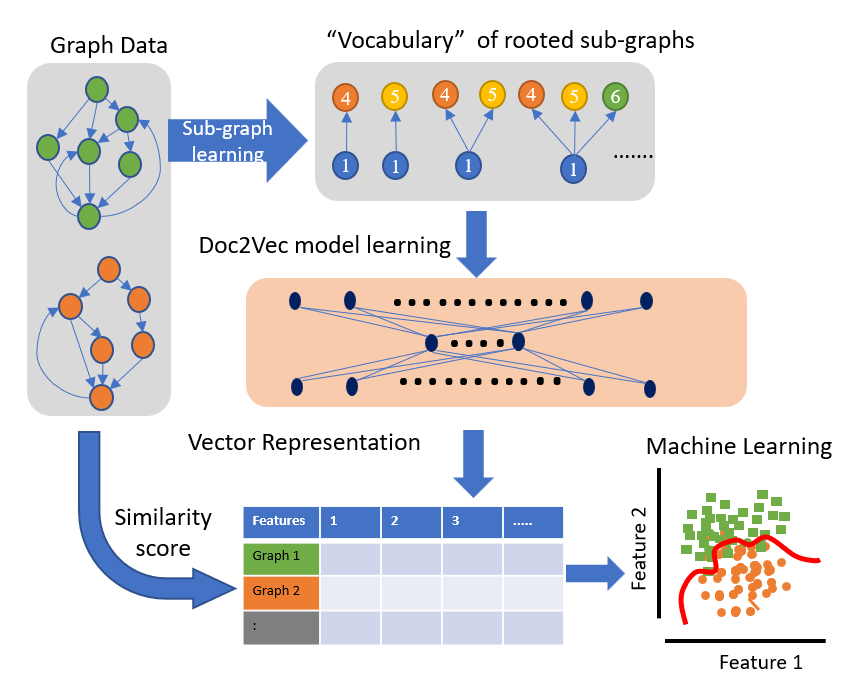
\includegraphics[width=0.9\columnwidth]{figures/Graph_embedding/Gaph2Vec.png}}
\caption{Graph2Vec pipeline overview}\label{fig: G2V}
\end{figure}

\section{Sparse Representation and Dictionary Learning}

There has been a growing interest in the search for sparse representations of signals in recent years. In the field of computer vision it can be reasonably assumed that image patches do not populate or sample the whole input domain\cite{Elad2010}. Sparse coding is a representation learning method which aims to find a sparse representation of an  $n$ dimensional input signal $y_i \in \mathbb{R}^n $ in the form of a sparse linear combination, such that the reconstructed data is $\tilde{y_i} = \alpha_{i,1} d_1 + \alpha_{i,2} d_2 + \cdots + \alpha_{i,K} d_K$. Where $\alpha_i \in \mathbb{R}^K$ is the the sparse vector and  $d_i \in \mathbb{R}^n $ are the dictionary elements (atoms) of a Dictionary $\mathbf{D}$. Sparse representation algorithms optimize  (\ref{eq1}) with a $l_0$ regularization term:

\begin{equation}
    \label{eq1}
    \argmin_{D,\alpha}||\mathbf{Y}-\mathbf{D} \mathbf{ \alpha }||_2^2  \;\; s.t.\;\; \forall i, || \alpha_i||_0 \leq S,
\end{equation}

\noindent where $\mathbf{Y}=[y_1,y_2,.., y_N] \in \mathbb{R}^{n\times N}$ denotes the $N$ number of input signals, $ \mathbf{D} = [d_1,d_2,\ldots,d_K] \in \mathbb{R}^{n \times K}$ is the learned dictionary of size $K$, $\mathbf{ \alpha } = [\alpha_1,\alpha_2,\ldots,\alpha_N ] \in \mathbb{R}^{K \times N}$ is the sparse representation of the input signal, and $S$ is the sparsity constraint of $\alpha_i$ (maximum number of non-zero elements). Usually  $K > n$, in which case the dictionary is called over-complete. If $K = n$ the dictionary is called complete and if $K < n$ it is called under-complete.

Equation (\ref{eq1}) can be solved by alternating between the following two stages. First, sparse coding is to calculate $\alpha$ with a fixed over-complete dictionary $D$. Second, dictionary learning is performed to update $D$ with a fixed $\alpha$. K-means Singular Value Decomposition (K-SVD)\cite{Aharon2006, Rubinstein2013} has emerged as an effective and popular algorithm for sparse representation tasks. K-SVD first initializes a random dictionary. It then alternates between the two stages by utilizing Orthogonal Matching Pursuit (OMP)\cite{Pati1993, Davis1997} for the sparse coding and generalized k-means with Singular Value Decomposition (SVD) for the dictionary update. K-SVD efficiently learns an over-complete dictionary and has been effectively utilized for tasks including de-noising, restoration, and classification.

For classification tasks, in order to improve the performance a more discriminatory representation is required. Jiang \textit{et al.}\cite{Jiang2011, Jiang2013} have presented a Label Consistent K-SVD (LC-KSVD) algorithm as an extension of the K-SVD framework, which is a supervised learning algorithm to learn a compact and discriminative dictionary. In LC-KSVD, class-specific dictionary elements are trained separately as an initialization and then combined to learn a discriminative dictionary. A label consistent constraint called \say{discriminative sparse-code error}, reconstruction error and classification error terms are combined to structure a unified objective function to optimize the discriminated dictionary. Due to the class constraints in the sparse coding and dictionary update stages, the input data will forced to be mapped to the dedicated dictionary atoms according to the label information. Consequently in the sparse dictionary domain, a majority of the input signals will be projected to a subspace belonging to a certain class. Hence, a lower order classifier can be trained for the classification. 

Traditional dictionary learning models do not take into account the class imbalances of the training data. Hence the dictionary atoms can be biased towards the larger class. Therefore to address the class imbalances and the structure, a separate dictionary learning algorithm is also employed. Frozen dictionary learning modifies the dictionary learning process as a hierarchical structure to learn a dictionary that can effectively model imbalanced datasets\cite{Carroll2017}. In this algorithm, first, the dictionary learning step is carried out using the K-SVD algorithm on \say{normal} training data. Then the learned dictionary elements are frozen (held constant) and the dictionary is augmented with additional elements by dictionary elements is trained again on abnormalities. This process is repeated for all the remaining classes, by keeping the previously learned dictionaries frozen. The frozen elements of the dictionary represent the \say{normal} aspects of the data, hence the new elements (non-frozen) learn to represent the anomalous aspects of the data that are not present in the \say{normal} data. The frozen dictionary approach could be generally used and applied to the problems including data with or without abnormalities.


\section{Feature Ranking}

eature Ranking (FR) is an essential part of the machine learning pipeline to identify, reduce, remove, or craft features that benefits ML performance and reduce the cost of the operations. In general, FR methods evaluate features by looking at the amount of information they provide and ranking them accordingly so that the most relevant and complementary features can be used in ML training. There are three main categories of methods for FR algorithms: Filter methods (FM), Wrapper methods (WM), and Embedded methods (EM). The FR methods can be further classified as \emph{myopic} and \emph{non-myopic}. Whereas\emph{myopic} methods only evaluate the feature by itself,\emph{non-myopic} methods take into the consideration of interrelationship between the features. Several surveys outline the current state-of-the-art in feature assessment techniques\cite{Uthman2020, Sangodiah2014, Effrosynidis2021, Jovic2015}. A summary of the method's pros and cons are shown in fig.\ref{fig: FR_methods}.

\begin{figure}[!t]
    \centering
    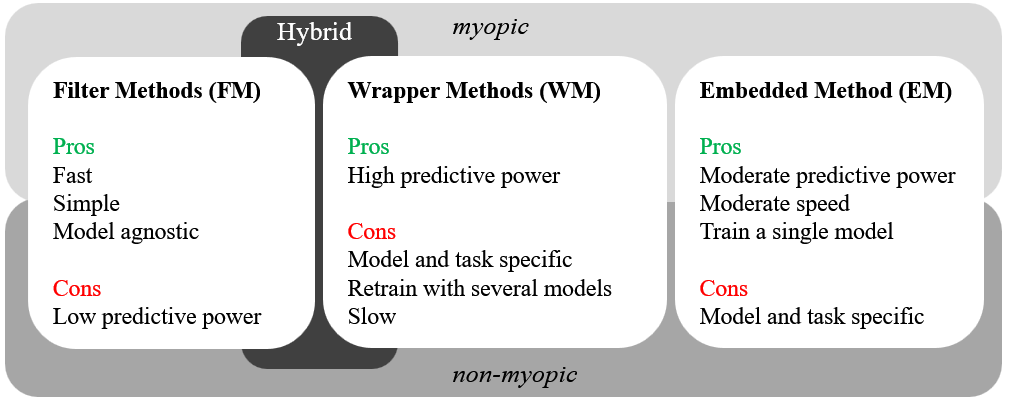
\includegraphics[width=12cm]{figures/eng694/FR_methods.png}
     \caption{Classification of the FR methods and summary of pros and cons}\label{fig: FR_methods}
\end{figure}


In FM, intrinsic properties are evaluated to determine the relevance of the feature. FM methods are generally computationally inexpensive and do not depend on the ML model since the evaluation is done independently. In WM the feature ranking is tied to the ML model performance. This method is more computationally expensive than the FM as it needs to train multiple ML models to identify which features contribute more. WM is model- and task-specific and, as a result, gives better results. However, WM has to be performed again for a different task or a model. EM is similar to WM, however, it performs the feature selection while the ML model is trained. Therefore, time is saved by avoiding training multiple models by sacrificing performance compared to WM\@. EM is also model and task-specific.  

The proposed SR-based methods can be considered as \textit{non-myopic} and a hybrid of FM and EM concepts. To calculate the two metrics, dictionary learning has to be carried out (like EM), which is more computationally expensive than the typical FM\@. However, these metrics do not depend on any ML methods so these FR scores can be used in many applications, unlike EM methods. Furthermore, the proposed metrics do not even have to depend on any particular SR method. However, using a discriminatory dictionary learning and (semi-) supervised SR method would be able to improve the interpretation ability of the data. Since the atoms are a subspace of the original feature space when atoms are learned it takes into account the relationship between all the features hence, these metrics are \textit{non-myopic}. Another main advantage is the ability to decompose the feature importance according to each class with supervised dictionary learning methods. Also, the learned dictionary is not wasted as the dictionary and the calculated sparse coefficients can be used for the training of classifiers in the next stages of the machine learning pipeline. 

Chang and Lin\cite{Chang2008} conducted FR using the weights of the linear SVM\@. Compared with a variant of Fisher-score\cite{Chang2011} (F-score) method, their method showed improved performance. However, it can be only used with a linear SVM\@. Jong, et al.\cite{Jong2004}, proposed an ensemble feature ranking (EFR) algorithm that aggregates results of multiple FR algorithms to gain higher performance. 

Relieff\cite{Kononenko1997} and mRMR\cite{Ding2005} are two commonly used FR algorithms. Both the methods can be considered as \textit{non-myopic} FM algorithms. Zhang et al.\cite{Zhang2019} implemented a novel SR-based feature assessment method called SRDA, where they employ both SR and information theory to identify dependencies and redundancies of the salient features. In this work, they evaluate the learned dictionary atoms (new features) for redundancy and complementary properties. In our work, we try to evaluate the original input features, not the derived sparse features. However, they provide some interesting frameworks for selecting candidate sparse features.

In recent years several deep learning methods have been proposed that achieve high accuracy for data sets. However, deep learning methods lack an intuitive relationship between the learned features and the input layer. Also, they require large computational resources for training and testing. It can be seen that almost all methods that have been used are some form of deep architecture. Usage of deep networks is popular due to the high performance and ability to learn features automatically\cite{Li2019}. We would urge readers to get familiarized with our previous work\cite{Liyanage2020} for a detailed discussion about the advantages of the SR methods concerning deep learning methods.

\section{Hyperbolic Space}